% =====================================================================
%  Lei de Zipf nas manchas urbanas do Nordeste brasileiro (GPW v4 + CCA)
%  Trabalho final — artigo de no máximo 3 páginas com elemento gráfico
%
%  Compilar com: pdflatex main -> bibtex main -> pdflatex main (2x)
%  Dados e figura: python analise_brasil.py ; python gerar_graficos_artigo.py
% =====================================================================
\documentclass[10pt,a4paper,twocolumn]{article}

\usepackage[utf8]{inputenc}
\usepackage[T1]{fontenc}
\usepackage[brazilian]{babel}
\usepackage[top=2cm,bottom=2cm,left=1.8cm,right=1.8cm,columnsep=0.65cm]{geometry}
\usepackage{graphicx}
\usepackage{amsmath,amssymb}
\usepackage{booktabs}
\usepackage{caption}
\usepackage{xcolor}
\usepackage{lmodern}
\usepackage{microtype}
\usepackage{flushend}
\usepackage{titlesec}
\usepackage{icomma}
\usepackage[colorlinks=true,allcolors=blue!70!black]{hyperref}

\captionsetup{font=small,labelfont=bf}

% Espaçamentos compactos e elegantes para seções e parágrafos
\titleformat{\section}{\large\bfseries}{\thesection}{0.7em}{}
\titlespacing*{\section}{0pt}{1.3ex plus .3ex minus .2ex}{0.7ex plus .2ex}
\newcommand{\rotuloparagrafo}[1]{#1.}
\titleformat{\paragraph}[runin]{\normalfont\bfseries}{\theparagraph}{0em}{\rotuloparagrafo}
\titlespacing*{\paragraph}{0pt}{0.7ex plus .2ex minus .1ex}{0.55em}

\pagestyle{empty}
\renewcommand{\topfraction}{0.88}
\renewcommand{\floatpagefraction}{0.75}

\begin{document}

% ---------------------------------------------------------------- cabeçalho e título
\twocolumn[
\begin{@twocolumnfalse}
\begin{center}
\IfFileExists{figs/unifor_logo.png}
  {
\includegraphics[height=1.4cm]{figs/unifor_logo.png}\par\vspace{0.2cm}}
  {\fbox{\parbox{5.5cm}{\centering\footnotesize\color{red}[inserir \texttt{figs/unifor\_logo.png}]}}\par\vspace{0.2cm}}

{\footnotesize\bfseries Universidade de Fortaleza (UNIFOR) \quad$\cdot$\quad Centro de Ciências Tecnológicas\\
Programa de Pós-Graduação em Informática Aplicada (PPGIA)\par}

\vspace{0.35cm}
{\LARGE\bfseries A lei de Zipf nas manchas urbanas do Nordeste brasileiro\par}
\vspace{0.18cm}
{\large Cidades definidas pelo \emph{City Clustering Algorithm} sobre o GPW v4, comparadas aos municípios\par}
\vspace{0.25cm}
{\normalsize\textbf{Thiago de Oliveira Sampaio}\par}
{\footnotesize Mestrado em Informática Aplicada, pesquisa de dissertação\par}
\vspace{0.35cm}
\end{center}

\begin{quote}\small
\noindent\textbf{Resumo.}
A lei de Zipf afirma que a população da cidade de posto $r$ decai como $S(r)\propto r^{-\alpha}$, com $\alpha=1$. Testá-la exige uma definição de cidade independente das fronteiras municipais, mas a definição por densidade do \emph{City Clustering Algorithm} (CCA) depende de dois parâmetros livres, o limiar de densidade $D^{*}$ e a distância de ligação $\ell$. Aplicamos o CCA ao raster de população GPW v4 (2020) do Brasil, varremos $15\,000$ pares $(D^{*},\ell)$ e escolhemos o par em que as 50, 100 e 200 maiores manchas ficam mais próximas de Zipf. Com $D^{*}=1\,450$\,hab/km$^{2}$ e $\ell=1{,}8$\,km, as $4\,702$ manchas do país seguem Zipf com precisão notável: $\alpha$ entre $0{,}99$ e $1{,}00$ no topo e $\alpha=1{,}00\pm0{,}04$ na cauda ajustada por máxima verossimilhança. Os municípios do Censo 2022 não seguem ($\alpha=0{,}91$, lei de potência rejeitada). No Nordeste, com a mesma definição de cidade, a cauda das $1\,729$ manchas é compatível com Zipf ($\alpha=0{,}92\pm0{,}05$), mas o topo não: as nove maiores manchas são as nove capitais estaduais, maiores do que Zipf prevê, e em nenhum dos pares de parâmetros com $\ell$ acima da resolução da grade o topo do \emph{ranking} regional se ajusta a Zipf. A lei de Zipf é uma propriedade do sistema urbano nacional que a rede de capitais do Nordeste não reproduz em escala regional.

\vspace{0.15cm}
\noindent\textbf{Palavras-chave:} lei de Zipf, \emph{City Clustering Algorithm} (CCA), GPW v4, Nordeste, rede urbana, estimador de Hill.
\end{quote}
\vspace{0.35cm}
\end{@twocolumnfalse}
]

% ---------------------------------------------------------------- problema
\section{Qual é o problema?}

Cidades não são objetos naturalmente delimitados. No Brasil, a população é
divulgada por município, e o município é uma unidade política: a metrópole do
Recife está repartida entre Recife, Olinda, Jaboatão dos Guararapes e outros
municípios, enquanto muitos municípios do sertão somam uma sede pequena e uma
grande área rural. Qualquer lei estatística sobre o tamanho das cidades depende,
portanto, de uma escolha prévia que normalmente fica implícita.

A \textbf{lei de Zipf}~\cite{zipf1949} é o exemplo canônico dessa dependência.
Na forma de posto e tamanho, a população $S$ da cidade de posto $r$ obedece
%
\begin{equation}
S(r) \;\propto\; r^{-\alpha}, \qquad \alpha = 1,
\label{eq:zipf}
\end{equation}
%
o que equivale a uma densidade $p(x)\propto x^{-\gamma}$ e a uma lei de
Pareto $P(X\geq x)\propto x^{-\zeta}$, com $\zeta=\gamma-1=1/\alpha$. Zipf é o
caso $\gamma=2$ dessa família de leis de potência~\cite{newman2005}. Para os
municípios brasileiros, Moura Jr. e Ribeiro~\cite{moura2006} estudaram a lei de
Zipf com dados censitários.

Rozenfeld \emph{et al.}~\cite{rozenfeld2008,rozenfeld2011} mostraram que o
expoente medido muda quando as cidades deixam de ser fronteiras legais e
passam a ser aglomerados construídos a partir da densidade, e propuseram o
\emph{City Clustering Algorithm} (CCA) como essa definição. O mesmo
agrupamento entra no estudo de emissões de CO$_2$~\cite{oliveira2014} e de
mobilidade e criminalidade~\cite{caminha2017}. O CCA, porém,
troca as fronteiras por dois parâmetros: o limiar $D^{*}$, acima do qual uma
célula é urbana, e a distância $\ell$ abaixo da qual duas células urbanas
pertencem à mesma mancha. Fixá-los por convenção deixa o expoente refém de
uma escolha arbitrária.

Este trabalho responde a três perguntas. \textbf{(i)} Existe um par
$(D^{*},\ell)$ em que as manchas urbanas do Brasil seguem Zipf, e quão sensível
é o expoente a essa escolha? \textbf{(ii)} Com a mesma definição de cidade, o
Nordeste segue Zipf? \textbf{(iii)} O que muda quando, em vez de manchas, se
usam municípios?

% ---- figura
\begin{figure*}[t]
\centering
\IfFileExists{figs/zipf.pdf}
  {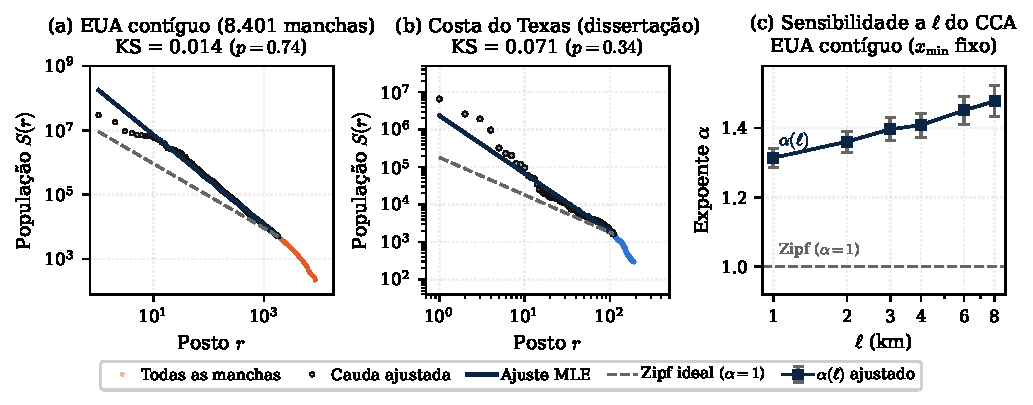
\includegraphics[width=\textwidth]{figs/zipf.pdf}}
  {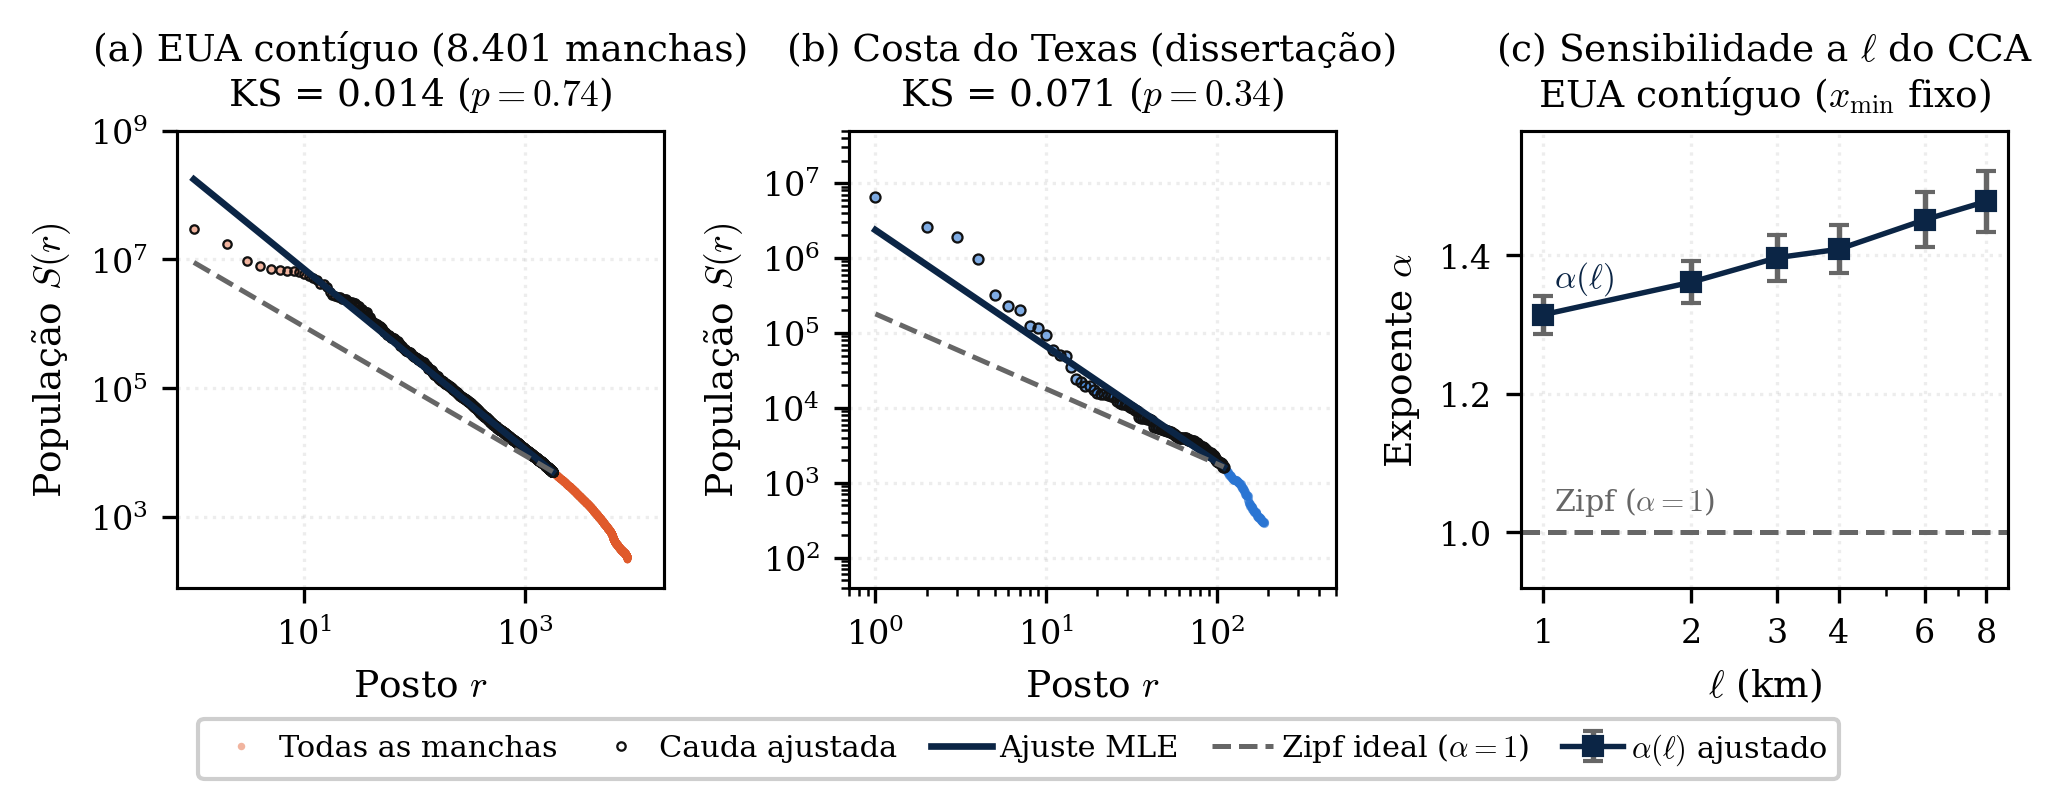
\includegraphics[width=\textwidth]{figs/zipf.png}}
\caption{\textbf{Manchas urbanas do Nordeste e sensibilidade do expoente.} \textbf{(a)} Centroides das $1\,729$ manchas do Nordeste no par calibrado para o Brasil ($D^{*}=1\,450$\,hab/km$^{2}$, $\ell=1{,}8$\,km); a área e a cor dos círculos crescem com a população. \textbf{(b)} População contra o posto no Nordeste: manchas do CCA (laranja) e municípios do Censo 2022 (cinza). Tracejado: Zipf, $S_1/r$, com $S_1$ a maior mancha; reta azul: ajuste de Clauset, Shalizi e Newman das manchas ($x\geq 10\,439$\,hab, $n=414$). \textbf{(c)} Expoente de Hill das $N$ maiores manchas contra $D^{*}$, com $\ell=1{,}8$\,km, no Brasil (preto) e no Nordeste (laranja); a linha vertical marca o $D^{*}$ calibrado.}
\label{fig:zipf}
\end{figure*}

% ---------------------------------------------------------------- método
\section{O que foi feito}

\paragraph{Dados} A população vem do \emph{Gridded Population of the World} v4
(GPW v4, revisão 11)~\cite{gpw4}, um raster de contagem de pessoas para 2020
com resolução de 30 segundos de arco ($\approx 0{,}93$\,km), que redistribui
os dados censitários numa grade regular. As células fora do Brasil e o pertencimento de cada célula ao Nordeste são definidas pelas malhas do país e das
nove unidades da federação do Nordeste, obtidas na API de malhas do
IBGE~\cite{ibgemalhas}. O recorte tem $215{,}8$ milhões de habitantes, dos
quais $59{,}5$ milhões no Nordeste. Para a comparação administrativa, usamos
a população dos $5\,570$ municípios no Censo 2022~\cite{ibge2022}, dos quais
$1\,794$ no Nordeste.

\paragraph{Definição de cidade (CCA)} Uma célula é urbana quando sua densidade
supera $D^{*}$, com a área da célula corrigida pelo fator $\cos(\mathrm{lat})$.
Duas células urbanas pertencem à mesma mancha quando a distância haversine, que é uma equação matemática usada para calcular a distância mais curta (distância ortodrômica) entre dois pontos na superfície de uma esfera, considerando a curvatura da Terra,
entre os seus centros é menor que $\ell$, e a relação é transitiva. O CCA roda
sobre o Brasil inteiro, e uma mancha é do Nordeste quando a maior parte da sua
população está na região. Assim as divisas estaduais não cortam manchas.

\paragraph{Varredura de parâmetros} Varremos $D^{*}=10, 20, \dots,
3\,000$\,hab/km$^{2}$ e $\ell=100, 200, \dots, 5\,000$\,m, num total de
$15\,000$ pares. Com $\ell$ fixo, as células urbanas para um limiar contêm as
de qualquer limiar maior. As células são então ativadas em ordem decrescente
de densidade e unidas, por uma estrutura de união e
busca~\cite{tarjan1975}, às vizinhas já ativas a menos de $\ell$. Quando a
densidade cruza um valor da grade, as manchas presentes são exatamente as do
CCA com aquele $D^{*}$, e uma única passada por $\ell$ produz os 300 limiares.
Como conferência, com $\ell=1{,}4$\,km o CCA no Brasil equivale à rotulagem
com vizinhança de 8 células, e as duas dão as mesmas $6\,088$ manchas para
$D^{*}=1\,000$\,hab/km$^{2}$.

\paragraph{Expoente e critério} Em cada par, o expoente das $N$ maiores
manchas é estimado pelo método de Hill~\cite{hill1975},
$\hat\alpha_N = \frac{1}{N-1}\sum_{i\leq N}\ln(S_i/S_N)$, para $N=50$, $100$
e $200$. Se as manchas seguem Zipf, $\hat\alpha_N\approx 1$ para qualquer $N$.
O par escolhido minimiza o pior desvio,
$\Delta = \max_N |\hat\alpha_N - 1|$, entre os pares com
$\ell\geq\ell_{\min}=1{,}4$\,km. Abaixo da diagonal entre centros de células
vizinhas ($\approx 1{,}3$\,km), o CCA deixa de ligar células adjacentes e
produz manchas fragmentadas pela própria grade.

\paragraph{Ajuste da cauda} A cauda é ajustada pelo método de Clauset,
Shalizi e Newman (CSN)~\cite{clauset2009}: $\gamma$ por máxima verossimilhança
no ramo $x\geq x_{\min}$, $x_{\min}$ pela menor distância de
Kolmogorov--Smirnov (KS) e bondade de ajuste por \emph{bootstrap} com 200
réplicas, em que $p>0{,}1$ significa que a lei de potência \textbf{não é
rejeitada}. A lei de potência é comparada às alternativas lognormal,
exponencial e truncada pela razão de verossimilhança de
Vuong~\cite{vuong1989,alstott2014}.

% ---------------------------------------------------------------- resultados
\section{Resultados e conclusões}

\paragraph{Brasil: Zipf nas manchas, não nos municípios} O par calibrado é
$D^{*}=1\,450$\,hab/km$^{2}$ e $\ell=1{,}8$\,km, com $\hat\alpha_{50}=0{,}99$,
$\hat\alpha_{100}=1{,}00$, $\hat\alpha_{200}=1{,}00$ e $\Delta=0{,}007$. As
$4\,702$ manchas somam $151$ milhões de habitantes, $70\%$ da população. A
escolha é pouco sensível: $5\,566$ dos $11\,100$ pares com $\ell\geq\ell_{\min}$
têm $\Delta<0{,}10$, com $D^{*}$ de $90$ a $3\,000$\,hab/km$^{2}$, e
$\hat\alpha_{100}$ fica entre $0{,}96$ e $1{,}33$ em toda essa parte da grade
(Fig.~\ref{fig:zipf}c, em preto). O ajuste CSN escolhe $x_{\min}=28\,777$
habitantes ($n=596$) e dá $\alpha=1{,}00\pm0{,}04$, com KS${}=0{,}021$ abaixo
do valor crítico de $0{,}056$ e $p=0{,}47$. A lei de potência é muito melhor
que a exponencial ($R=4{,}5$, $p<10^{-5}$) e não se distingue da lognormal nem
da truncada ($p=0{,}99$ e $0{,}48$). São Paulo ($20{,}0$\,M) e Rio de Janeiro
($8{,}9$\,M) estão na razão de $0{,}45$, perto do $0{,}5$ de Zipf.
Os $5\,570$ municípios dão outro resultado: $\alpha=0{,}91\pm0{,}02$ na cauda
($x_{\min}=22\,393$), com $p=0{,}045$, o que \textbf{rejeita} a lei de
potência, e um topo achatado, com $\hat\alpha_{50}=0{,}70$.

\paragraph{Nordeste: a cauda segue Zipf, o topo não} Com a definição nacional
de cidade, o Nordeste tem $1\,729$ manchas, que somam $35{,}5$ milhões de
habitantes, $60\%$ da população da região (Fig.~\ref{fig:zipf}a). A cauda é
compatível com Zipf: o ajuste CSN dá $\alpha=0{,}92\pm0{,}05$ acima de
$x_{\min}=10\,439$ habitantes ($n=414$), com KS${}=0{,}026$ abaixo do crítico
de $0{,}067$ e $p=0{,}45$. O topo, porém, não segue (Fig.~\ref{fig:zipf}b).
As nove maiores manchas são as nove capitais estaduais: Recife ($3{,}47$\,M),
Fortaleza ($3{,}35$\,M) e Salvador ($3{,}10$\,M), quase empatadas, e depois São
Luís ($1{,}30$\,M), Natal ($1{,}23$\,M), Maceió ($1{,}07$\,M), João Pessoa
($1{,}05$\,M), Teresina ($0{,}98$\,M) e Aracaju ($0{,}83$\,M). Zipf daria à
segunda mancha metade da primeira, e não $97\%$, e à nona $0{,}39$\,M, menos
da metade de Aracaju. O primeiro centro não capital, Feira de Santana
($0{,}53$\,M), vem só em décimo. Esse degrau aparece no estimador:
$\hat\alpha_{50}=1{,}18$, contra $\hat\alpha_{100}=0{,}93$ e
$\hat\alpha_{200}=0{,}95$. O degrau não depende da definição de cidade: em
todos os $11\,100$ pares com $\ell\geq\ell_{\min}$, $\hat\alpha_{50}$ do
Nordeste fica entre $1{,}07$ e $1{,}34$ (Fig.~\ref{fig:zipf}c, em laranja). A
calibração feita só com o Nordeste confirma isso: o melhor par
($D^{*}=110$\,hab/km$^{2}$, $\ell=3{,}4$\,km) ainda tem $\Delta=0{,}07$ e põe
$81\%$ da população da região em manchas, o que indica que o limiar já inclui
ocupação não urbana.

\paragraph{Manchas e municípios} A diferença entre as duas definições é
maior nas metrópoles. A mancha do Recife tem $3{,}47$ milhões de habitantes e
o município, $1{,}49$ milhão: no \emph{ranking} municipal, Recife é o terceiro
do Nordeste, atrás de Fortaleza e Salvador; no de manchas, é o primeiro. Na
cauda, os $1\,794$ municípios dão $\alpha=0{,}74\pm0{,}03$, bem abaixo de 1, o
que é esperado quando municípios grandes em área agregam sede e zona rural.

\paragraph{Limitações} O GPW de 2020 é uma extrapolação dos censos de 2010, e
soma $59{,}5$ milhões no Nordeste contra $54{,}7$ milhões no Censo 2022; a
comparação entre manchas e municípios mistura, portanto, duas fontes e dois
anos. A resolução de $\approx 1$\,km limita $\ell$ por baixo. O critério
$\Delta$ é uma escolha: outro conjunto de $N$ moveria o par calibrado dentro
da ampla região de $\Delta$ pequeno, sem mudar as conclusões, que valem em
toda a grade. A análise usa um único ano e não diz nada sobre a dinâmica de
crescimento.

\paragraph{Conclusão} Com cidades definidas pela densidade, o Brasil segue a
lei de Zipf com precisão, em uma ampla faixa de parâmetros; com cidades
definidas por municípios, não segue. O Nordeste segue Zipf nas cidades médias
e pequenas, mas não no topo: sua rede urbana é organizada em torno das nove
capitais estaduais, maiores do que Zipf prevê e com três metrópoles de porte
semelhante. A lei de Zipf é, assim, uma propriedade do sistema urbano
nacional, em que essas capitais ocupam posições intermediárias, e não de cada
região.

% ---------------------------------------------------------------- refs
\bibliographystyle{unsrt}
\bibliography{referencias}

\end{document}
